\chapter{Result}\label{result}
The result from the multiple runs we have gotten are shown in the different figures. Figure \ref{fig:smallResult} shows the spread and coverage from the simulation of the small graph. As we can see, the four different algorithm had little difference. The y-akses shows us the average coverage after 50 runs, and the x-akses gives us how many seed node was selected. We can see from figure \ref{fig:smallResult}, figure \ref{fig:mediumResult} and figure \ref{fig:largeResult} that the resulted coverage was around 0.3-0.45. The smaller graph would result in a smaller spread, while larger graph results in large spread. Figure \ref{fig:smallResult} have a more linear increase as the seed nodes increased. Figure \ref{fig:mediumResult} and Figure \ref{fig:largeResult} on the other hand, had an massive increase in coverage after the addition of the second seed node, then the increase slowed down drastically. 

The network that we ran our simulation on, resulted in a degree distribution as Figure \ref{fig:smallDegree}, Figure \ref{fig:mediumDegree}, and Figure \ref{fig:largeDegree}. We can see that there are one vertex with high degree, while the majority of the nodes have a small degree. 


We can see that the greedy algorithm performed better then the other algorithm for the large and medium graph, except the random algorithm for the large graph, which was the best.


Our result as a table:

\begin{figure}[t]
	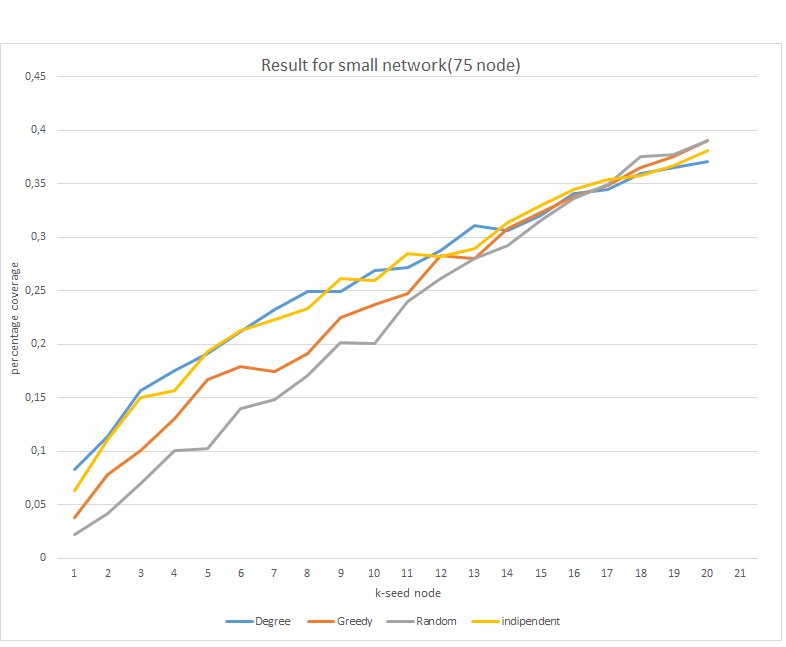
\includegraphics[width=0.7\textwidth]{small_result}
	\caption{The result from the small graph} 
	\label{fig:smallResult}
\end{figure}

\begin{table}[b]
\begin{center}
\begin{tabular}{|l|l|l|l|l|}
\hline
k & Degree 			& Greedy 			& Random 			& Indipendent \\
\hline
1& 0.0832			& 0.0381333333333 	& 0.0224			& 0.634666666667 \\
2&0.114133333333	& 0.0778666666667	& 0.0413333333333	& 0.110933333333 \\
3&0.157066666667	& 0.100533333333	& 0.0696			& 0.149866666667 \\
4&0.175733333333	& 0.130666666667	& 0.100266666667	& 0.156266666667 \\
5&0.190933333333	& 0.166666666667	& 0.102933333333	& 0.193066666667 \\
6&0.212				& 0.178933333333	& 0.139466666667	& 0.212266666667 \\
7&0.232533333333	& 0.174666666667	& 0.148533333333	& 0.2232 \\
8&0.2488			& 0.1912			& 0.1704			& 0.233333333333 \\
9&0.249066666667	& 0.225066666667	& 0.201333333333	& 0.261066666667 \\
10&0.2688			& 0.237333333333	& 0.200266666667	& 0.2592 \\
11&0.271466666667	& 0.246933333333	& 0.239466666667	& 0.285066666667 \\
12&0.287733333333	& 0.2832			& 0.261066666667	& 0.281866666667 \\
13&0.310933333333	& 0.280266666667	& 0.279733333333	& 0.2896 \\
14&0.306133333333	& 0.308 			& 0.292533333333	& 0.313866666667 \\
15&0.320266666667	& 0.322666666667	& 0.3152			& 0.329066666667 \\
16&0.3408			& 0.338133333333 	& 0.336				& 0.3448 \\
17&0.344533333333	& 0.348266666667 	& 0.3496			& 0.354133333333 \\
18&0.359733333333	& 0.348266666667	& 0.375466666667	& 0.3576 \\
19&0.3648			& 0.375733333333 	& 0.377333333333	& 0.366933333333 \\
20&0.370933333333	& 0.389866666667	& 0.3904			&  0.381333333333 \\
\hline
\end{tabular}
\end{center}
\caption{Result from small graph}
\end{table}




\begin{figure}[t]
	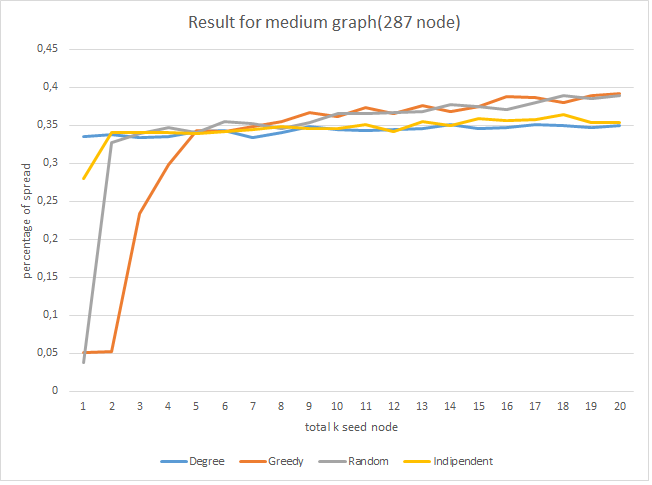
\includegraphics[width=0.7\textwidth]{medium_result}
	\caption{The result from the medium graph} 
	\label{fig:mediumResult}
\end{figure}

\begin{table}[b]
\begin{center}
\begin{tabular}{|l|l|l|l|l|}
\hline
k & Degree 			& Greedy 			& Random 			& Indipendent \\
\hline
1&0.334773519164	&0.0506620209059	&0.0384668989547&0.279790940767\\
2&0.337421602787	&0.0529616724739	&0.327456445993	&0.340069686411\\
3&0.334216027875	&0.23393728223		&0.339442508711	&0.340975609756\\
4&0.335400696864	&0.298048780488		&0.34668989547	&0.341324041812\\
5&0.341742160279	&0.342926829268		&0.340557491289	&0.339930313589\\
6&0.34362369338		&0.341672473868		&0.354773519164	&0.341463414634\\
7&0.334076655052	&0.348571428571		&0.352055749129	&0.345156794425\\
8&0.341324041812	&0.355191637631		&0.346550522648	&0.348780487805\\
9&0.347944250871	&0.366968641115		&0.353867595819	&0.345644599303\\
10&0.344390243902	&0.362369337979		&0.365156794425	&0.345365853659\\
11&0.343554006969	&0.373449477352		&0.365783972125	&0.350871080139\\
12&0.34425087108	&0.366271777003		&0.36668989547	&0.341881533101\\
13&0.346132404181	&0.375609756098		&0.368432055749	&0.354912891986\\
14&0.351358885017	&0.368710801394		&0.377979094077	&0.349337979094\\
15&0.345714285714	&0.374285714286		&0.37456445993 	&0.359442508711\\
16&0.347804878049	&0.38850174216		&0.371567944251	&0.355818815331\\
17&0.351010452962	&0.386620209059		&0.379721254355	&0.357909407666\\
18&0.350383275261	&0.380766550523		&0.389128919861	&0.364320557491\\
19&0.347386759582	&0.388989547038		&0.385714285714	&0.354285714286\\
20&0.349268292683	&0.391986062718		&0.389477351916	&0.353658536585\\
\hline
\end{tabular}
\end{center}
\caption{Result from medium graph}
\end{table}



\begin{figure}[t]
	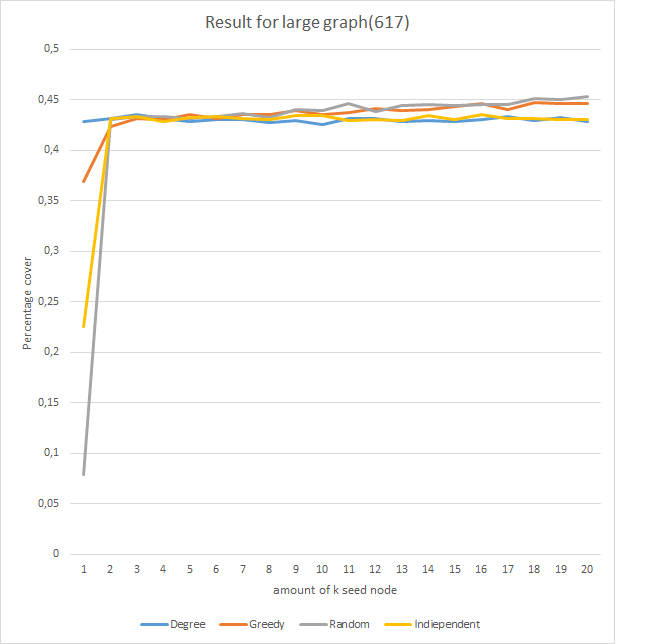
\includegraphics[width=0.65\textwidth]{large_result}
	\caption{The result from the large graph} 
	\label{fig:largeResult}
\end{figure}


\begin{table}[b]
\begin{center}
\begin{tabular}{|l|l|l|l|l|}
\hline
k & Degree 			& Greedy 			& Random 			& Indipendent \\
\hline
1&0.428363047002	&0.368881685575&	0.0788330632091	& 0.225705024311\\
2&0.431993517018	&0.423857374392&	0.430696920583	&0.431928687196\\
3&0.435364667747	&0.431831442464&	0.433873581848	&0.433387358185\\
4&0.431150729335	&0.430470016207&	0.433614262561	&0.428849270665\\
5&0.42829821718		&0.435818476499&	0.431863857374	&0.432544570502\\
6&0.430275526742	&0.432025931929&	0.433614262561	&0.433776337115\\
7&0.430210696921	&0.435559157212&	0.436369529984	&0.431377633712\\
8&0.427487844408	&0.435170178282&	0.432414910859	&0.430923824959\\
9&0.429951377634	&0.439643435981&	0.440713128039	&0.434424635332	\\
10&0.425380875203	&0.435170178282&	0.439189627229	&0.435072933549\\
11&0.431280388979	&0.437471636953&	0.446612641815	&0.429692058347\\
12&0.431993517018	&0.441847649919&	0.438995137763	&0.431118314425\\
13&0.428200972447	&0.439384116694&	0.444278768233	&0.429627228525\\
14&0.429529983793	&0.440842787682&	0.445316045381	&0.434586709887\\
15&0.428719611021	&0.443824959481&	0.444829821718	&0.431118314425\\
16&0.431118314425	&0.446126418152&	0.4456726094	&0.43510534846\\
17&0.433938411669	&0.440097244733&	0.445510534846	&0.43209076175\\
18&0.42982171799	&0.447066450567&	0.451280388979	&0.431345218801\\
19&0.432350081037	&0.446677471637&	0.450437601297	&0.431021069692\\
20&0.428784440843	&0.446839546191&	0.453452188006	&0.430632090762\\
\hline
\end{tabular}
\end{center}
\caption{result from large graph}
\end{table}

\begin{figure}[t]
	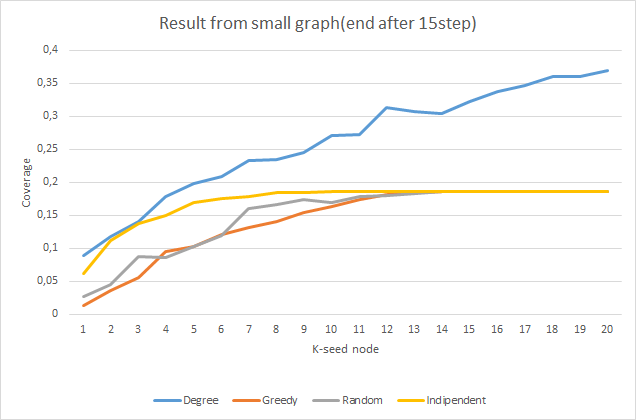
\includegraphics[width=0.65\textwidth]{step_small_result}
	\caption{The result from the small second simulation} 
	\label{fig:stepSmallResult}
\end{figure}

\begin{figure}[t]
	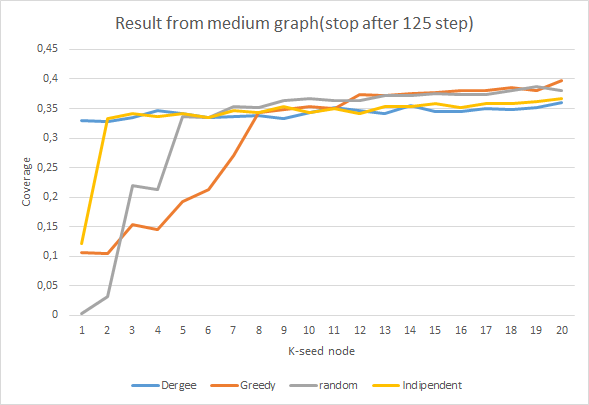
\includegraphics[width=0.65\textwidth]{step_medium_result}
	\caption{The result from the medium second simulation} 
	\label{fig:stepMediumResult}
\end{figure}

\begin{figure}[t]
	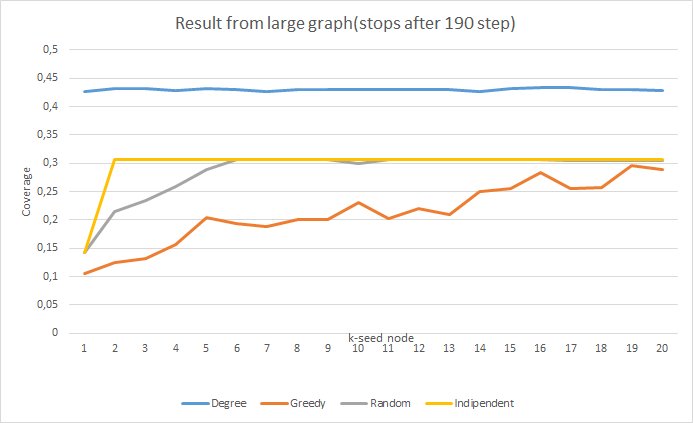
\includegraphics[width=0.65\textwidth]{step_large_result}
	\caption{The result from the large second simulation} 
	\label{fig:stepLargeResult}
\end{figure}


